\subsection{Contact Resistance}
\label{sec:test:contact}

\begin{figure}[!htb]
\begin{center}
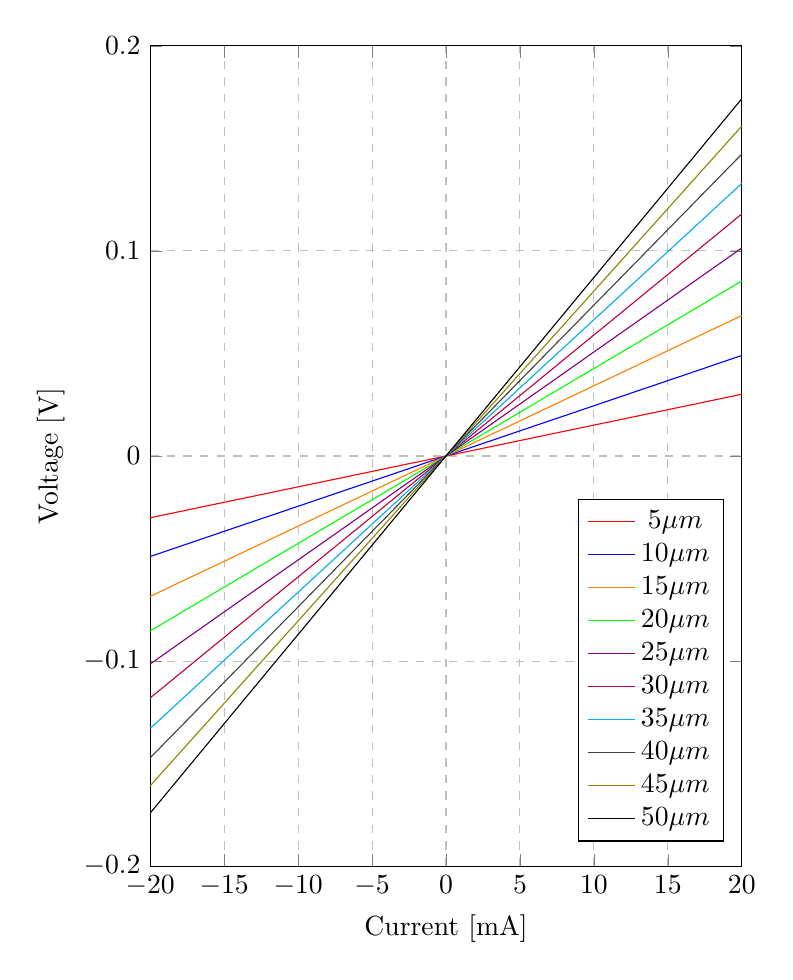
\begin{tikzpicture}

\begin{axis}[
    %title={Temperature dependence of CuSO$_4\cdot$5H$_2$O solubility},
    xlabel={Current [mA]},
    ylabel={Voltage [V]},
    height=12cm,
    width=0.75\textwidth,
    xmin=-20, xmax=20,
    ymin=-0.2, ymax=0.2,
    xtick={-20, -15, -10, -5, 0, 5, 10, 15, 20},
    ytick={-0.2, -0.1, 0, 0.1, 0.2},
    legend pos=south east,
    ymajorgrids=true,
    xmajorgrids=true,
    grid style=dashed,
]

\addplot[color=red]
  coordinates {
  (-20.000000000,-0.030106060)
  (-19.800000000,-0.029834320)
  (-19.600000000,-0.029502170)
  (-19.400000000,-0.029243770)
  (-19.200000000,-0.028904960)
  (-19.000000000,-0.028604000)
  (-18.800000000,-0.028321410)
  (-18.600000000,-0.027993270)
  (-18.400000000,-0.027730100)
  (-18.200000000,-0.027401190)
  (-18.000000000,-0.027122790)
  (-17.800000000,-0.026811620)
  (-17.600000000,-0.026515550)
  (-17.400000000,-0.026201050)
  (-17.200000000,-0.025873040)
  (-17.000000000,-0.025601530)
  (-16.800000000,-0.025270790)
  (-16.600000000,-0.025009270)
  (-16.400000000,-0.024675430)
  (-16.200000000,-0.024386870)
  (-16.000000000,-0.024089180)
  (-15.800000000,-0.023788190)
  (-15.600000000,-0.023492090)
  (-15.400000000,-0.023174160)
  (-15.200000000,-0.022900680)
  (-15.000000000,-0.022555040)
  (-14.800000000,-0.022285900)
  (-14.600000000,-0.021952910)
  (-14.400000000,-0.021677930)
  (-14.200000000,-0.021400330)
  (-14.000000000,-0.021074900)
  (-13.800000000,-0.020809100)
  (-13.600000000,-0.020466820)
  (-13.400000000,-0.020197590)
  (-13.200000000,-0.019878860)
  (-13.000000000,-0.019578650)
  (-12.800000000,-0.019280900)
  (-12.600000000,-0.018967320)
  (-12.400000000,-0.018688730)
  (-12.200000000,-0.018350630)
  (-12.000000000,-0.018089970)
  (-11.800000000,-0.017764520)
  (-11.600000000,-0.017494540)
  (-11.400000000,-0.017169810)
  (-11.200000000,-0.016848560)
  (-11.000000000,-0.016563480)
  (-10.800000000,-0.016233800)
  (-10.600000000,-0.015964600)
  (-10.400000000,-0.015660120)
  (-10.200000000,-0.015387690)
  (-10.000000000,-0.015047020)
  (-9.800000000,-0.014755250)
  (-9.600000000,-0.014452450)
  (-9.400000000,-0.014156350)
  (-9.200000000,-0.013884710)
  (-9.000000000,-0.013545790)
  (-8.800000000,-0.013270000)
  (-8.600000000,-0.012938530)
  (-8.400000000,-0.012656890)
  (-8.200000000,-0.012359900)
  (-8.000000000,-0.012042070)
  (-7.800000000,-0.011768720)
  (-7.600000000,-0.011444020)
  (-7.400000000,-0.011175730)
  (-7.200000000,-0.010848550)
  (-7.000000000,-0.010570180)
  (-6.800000000,-0.010258150)
  (-6.600000000,-0.009958734)
  (-6.400000000,-0.009645030)
  (-6.200000000,-0.009322094)
  (-6.000000000,-0.009053774)
  (-5.800000000,-0.008728319)
  (-5.600000000,-0.008459984)
  (-5.400000000,-0.008136192)
  (-5.200000000,-0.007836758)
  (-5.000000000,-0.007551670)
  (-4.800000000,-0.007221994)
  (-4.600000000,-0.006941887)
  (-4.400000000,-0.006613061)
  (-4.200000000,-0.006332992)
  (-4.000000000,-0.006019269)
  (-3.800000000,-0.005726597)
  (-3.600000000,-0.005432208)
  (-3.400000000,-0.005126086)
  (-3.200000000,-0.004852739)
  (-3.000000000,-0.004499509)
  (-2.800000000,-0.004230380)
  (-2.600000000,-0.003902373)
  (-2.400000000,-0.003620612)
  (-2.200000000,-0.003337186)
  (-2.000000000,-0.003018418)
  (-1.800000000,-0.002738350)
  (-1.600000000,-0.002417075)
  (-1.400000000,-0.002142058)
  (-1.200000000,-0.001826658)
  (-1.000000000,-0.001545745)
  (-0.800000000,-0.001210172)
  (-0.600000000,-0.000935144)
  (-0.400000000,-0.000618917)
  (-0.200000000,-0.000295114)
  (0.000000000,0.000014393)
  (0.200000000,0.000265850)
  (0.400000000,0.000592978)
  (0.600000000,0.000867126)
  (0.800000000,0.001190889)
  (1.000000000,0.001515501)
  (1.200000000,0.001771981)
  (1.400000000,0.002098289)
  (1.600000000,0.002375797)
  (1.800000000,0.002689450)
  (2.000000000,0.003003969)
  (2.200000000,0.003283158)
  (2.400000000,0.003615343)
  (2.600000000,0.003893689)
  (2.800000000,0.004206515)
  (3.000000000,0.004508429)
  (3.200000000,0.004800241)
  (3.400000000,0.005115563)
  (3.600000000,0.005393963)
  (3.800000000,0.005711809)
  (4.000000000,0.005995247)
  (4.200000000,0.006314762)
  (4.400000000,0.006609110)
  (4.600000000,0.006913514)
  (4.800000000,0.007238965)
  (5.000000000,0.007502181)
  (5.200000000,0.007823448)
  (5.400000000,0.008103450)
  (5.600000000,0.008420493)
  (5.800000000,0.008730789)
  (6.000000000,0.009020092)
  (6.200000000,0.009348963)
  (6.400000000,0.009619666)
  (6.600000000,0.009948456)
  (6.800000000,0.010237770)
  (7.000000000,0.010534610)
  (7.200000000,0.010828150)
  (7.400000000,0.011124960)
  (7.600000000,0.011443690)
  (7.800000000,0.011722030)
  (8.000000000,0.012061800)
  (8.200000000,0.012340910)
  (8.400000000,0.012650440)
  (8.600000000,0.012943140)
  (8.800000000,0.013217340)
  (9.000000000,0.013545230)
  (9.200000000,0.013822720)
  (9.400000000,0.014149000)
  (9.600000000,0.014432390)
  (9.800000000,0.014743560)
  (10.000000000,0.015047130)
  (10.200000000,0.015330470)
  (10.400000000,0.015651770)
  (10.600000000,0.015937700)
  (10.800000000,0.016263970)
  (11.000000000,0.016523850)
  (11.200000000,0.016839260)
  (11.400000000,0.017131820)
  (11.600000000,0.017448200)
  (11.800000000,0.017760760)
  (12.000000000,0.018047700)
  (12.200000000,0.018367980)
  (12.400000000,0.018640460)
  (12.600000000,0.018963390)
  (12.800000000,0.019250970)
  (13.000000000,0.019548710)
  (13.200000000,0.019865820)
  (13.400000000,0.020155860)
  (13.600000000,0.020482160)
  (13.800000000,0.020757970)
  (14.000000000,0.021079200)
  (14.200000000,0.021362600)
  (14.400000000,0.021677120)
  (14.600000000,0.021965590)
  (14.800000000,0.022248970)
  (15.000000000,0.022567780)
  (15.200000000,0.022856990)
  (15.400000000,0.023188540)
  (15.600000000,0.023463280)
  (15.800000000,0.023766000)
  (16.000000000,0.024078930)
  (16.200000000,0.024364800)
  (16.400000000,0.024676750)
  (16.600000000,0.024948250)
  (16.800000000,0.025265470)
  (17.000000000,0.025568180)
  (17.200000000,0.025881850)
  (17.400000000,0.026178650)
  (17.600000000,0.026475540)
  (17.800000000,0.026806030)
  (18.000000000,0.027079410)
  (18.200000000,0.027392230)
  (18.400000000,0.027663830)
  (18.600000000,0.027983480)
  (18.800000000,0.028297080)
  (19.000000000,0.028591360)
  (19.200000000,0.028921060)
  (19.400000000,0.029192690)
  (19.600000000,0.029517350)
  (19.800000000,0.029806520)
  (20.000000000,0.030110980)
    };
  \addlegendentry{$5\mu m$}

\addplot[color=blue]
  coordinates {
  (-20.000000000,-0.048996770)
  (-19.800000000,-0.048549300)
  (-19.600000000,-0.048018630)
  (-19.400000000,-0.047562660)
  (-19.200000000,-0.047049750)
  (-19.000000000,-0.046527550)
  (-18.800000000,-0.046080670)
  (-18.600000000,-0.045549230)
  (-18.400000000,-0.045090950)
  (-18.200000000,-0.044606440)
  (-18.000000000,-0.044098870)
  (-17.800000000,-0.043637680)
  (-17.600000000,-0.043117850)
  (-17.400000000,-0.042657830)
  (-17.200000000,-0.042136670)
  (-17.000000000,-0.041667780)
  (-16.800000000,-0.041167380)
  (-16.600000000,-0.040678030)
  (-16.400000000,-0.040190960)
  (-16.200000000,-0.039658600)
  (-16.000000000,-0.039228040)
  (-15.800000000,-0.038692710)
  (-15.600000000,-0.038251370)
  (-15.400000000,-0.037719120)
  (-15.200000000,-0.037228050)
  (-15.000000000,-0.036752810)
  (-14.800000000,-0.036238120)
  (-14.600000000,-0.035770520)
  (-14.400000000,-0.035244770)
  (-14.200000000,-0.034792240)
  (-14.000000000,-0.034274250)
  (-13.800000000,-0.033804890)
  (-13.600000000,-0.033304480)
  (-13.400000000,-0.032826050)
  (-13.200000000,-0.032365130)
  (-13.000000000,-0.031831030)
  (-12.800000000,-0.031368320)
  (-12.600000000,-0.030840460)
  (-12.400000000,-0.030379320)
  (-12.200000000,-0.029894030)
  (-12.000000000,-0.029391910)
  (-11.800000000,-0.028926890)
  (-11.600000000,-0.028422990)
  (-11.400000000,-0.027957240)
  (-11.200000000,-0.027428980)
  (-11.000000000,-0.026963870)
  (-10.800000000,-0.026462010)
  (-10.600000000,-0.025973090)
  (-10.400000000,-0.025494450)
  (-10.200000000,-0.024996570)
  (-10.000000000,-0.024529040)
  (-9.800000000,-0.024006890)
  (-9.600000000,-0.023556720)
  (-9.400000000,-0.023036190)
  (-9.200000000,-0.022551640)
  (-9.000000000,-0.022066540)
  (-8.800000000,-0.021542490)
  (-8.600000000,-0.021089950)
  (-8.400000000,-0.020562660)
  (-8.200000000,-0.020100880)
  (-8.000000000,-0.019592050)
  (-7.800000000,-0.019122890)
  (-7.600000000,-0.018620710)
  (-7.400000000,-0.018134670)
  (-7.200000000,-0.017686270)
  (-7.000000000,-0.017126190)
  (-6.800000000,-0.016674490)
  (-6.600000000,-0.016148100)
  (-6.400000000,-0.015681180)
  (-6.200000000,-0.015219530)
  (-6.000000000,-0.014709770)
  (-5.800000000,-0.014256400)
  (-5.600000000,-0.013726540)
  (-5.400000000,-0.013271610)
  (-5.200000000,-0.012756960)
  (-5.000000000,-0.012269120)
  (-4.800000000,-0.011782930)
  (-4.600000000,-0.011280870)
  (-4.400000000,-0.010803990)
  (-4.200000000,-0.010292600)
  (-4.000000000,-0.009841848)
  (-3.800000000,-0.009324592)
  (-3.600000000,-0.008856147)
  (-3.400000000,-0.008343101)
  (-3.200000000,-0.007826687)
  (-3.000000000,-0.007365859)
  (-2.800000000,-0.006839307)
  (-2.600000000,-0.006396058)
  (-2.400000000,-0.005872931)
  (-2.200000000,-0.005402779)
  (-2.000000000,-0.004907406)
  (-1.800000000,-0.004397748)
  (-1.600000000,-0.003934320)
  (-1.400000000,-0.003405306)
  (-1.200000000,-0.002948615)
  (-1.000000000,-0.002439780)
  (-0.800000000,-0.001985620)
  (-0.600000000,-0.001456592)
  (-0.400000000,-0.000995703)
  (-0.200000000,-0.000502852)
  (0.000000000,-0.000017567)
  (0.200000000,0.000492906)
  (0.400000000,0.000938607)
  (0.600000000,0.001455785)
  (0.800000000,0.001967918)
  (1.000000000,0.002426238)
  (1.200000000,0.002948468)
  (1.400000000,0.003399230)
  (1.600000000,0.003916400)
  (1.800000000,0.004416751)
  (2.000000000,0.004877617)
  (2.200000000,0.005377123)
  (2.400000000,0.005867376)
  (2.600000000,0.006355136)
  (2.800000000,0.006876527)
  (3.000000000,0.007315500)
  (3.200000000,0.007839410)
  (3.400000000,0.008294345)
  (3.600000000,0.008807332)
  (3.800000000,0.009323655)
  (4.000000000,0.009781969)
  (4.200000000,0.010321010)
  (4.400000000,0.010765050)
  (4.600000000,0.011288120)
  (4.800000000,0.011754830)
  (5.000000000,0.012236690)
  (5.200000000,0.012748030)
  (5.400000000,0.013216420)
  (5.600000000,0.013736090)
  (5.800000000,0.014192700)
  (6.000000000,0.014715830)
  (6.200000000,0.015184230)
  (6.400000000,0.015676130)
  (6.600000000,0.016169800)
  (6.800000000,0.016623860)
  (7.000000000,0.017157840)
  (7.200000000,0.017618750)
  (7.400000000,0.018153650)
  (7.600000000,0.018607670)
  (7.800000000,0.019081970)
  (8.000000000,0.019586570)
  (8.200000000,0.020048290)
  (8.400000000,0.020577160)
  (8.600000000,0.021030580)
  (8.800000000,0.021547760)
  (9.000000000,0.022030400)
  (9.200000000,0.022522310)
  (9.400000000,0.023018420)
  (9.600000000,0.023489350)
  (9.800000000,0.024012480)
  (10.000000000,0.024461710)
  (10.200000000,0.024980580)
  (10.400000000,0.025442910)
  (10.600000000,0.025972660)
  (10.800000000,0.026444360)
  (11.000000000,0.026932210)
  (11.200000000,0.027452770)
  (11.400000000,0.027904300)
  (11.600000000,0.028427430)
  (11.800000000,0.028897560)
  (12.000000000,0.029387750)
  (12.200000000,0.029882300)
  (12.400000000,0.030363260)
  (12.600000000,0.030880400)
  (12.800000000,0.031336240)
  (13.000000000,0.031872000)
  (13.200000000,0.032336100)
  (13.400000000,0.032842430)
  (13.600000000,0.033305820)
  (13.800000000,0.033769050)
  (14.000000000,0.034300590)
  (14.200000000,0.034751590)
  (14.400000000,0.035289540)
  (14.600000000,0.035746200)
  (14.800000000,0.036245700)
  (15.000000000,0.036740990)
  (15.200000000,0.037215330)
  (15.400000000,0.037726580)
  (15.600000000,0.038179740)
  (15.800000000,0.038706280)
  (16.000000000,0.039160420)
  (16.200000000,0.039676200)
  (16.400000000,0.040144260)
  (16.600000000,0.040653910)
  (16.800000000,0.041174480)
  (17.000000000,0.041634440)
  (17.200000000,0.042147420)
  (17.400000000,0.042603300)
  (17.600000000,0.043119440)
  (17.800000000,0.043612500)
  (18.000000000,0.044091690)
  (18.200000000,0.044599530)
  (18.400000000,0.045072350)
  (18.600000000,0.045598600)
  (18.800000000,0.046054390)
  (19.000000000,0.046566400)
  (19.200000000,0.047036710)
  (19.400000000,0.047545410)
  (19.600000000,0.048020520)
  (19.800000000,0.048482550)
  (20.000000000,0.049018070)

    };
  \addlegendentry{$10\mu m$}

\addplot[color=orange]
  coordinates {
  (-20.000000000,-0.068456910)
  (-19.800000000,-0.067766910)
  (-19.600000000,-0.067100920)
  (-19.400000000,-0.066389520)
  (-19.200000000,-0.065725360)
  (-19.000000000,-0.065033320)
  (-18.800000000,-0.064319760)
  (-18.600000000,-0.063671350)
  (-18.400000000,-0.062957310)
  (-18.200000000,-0.062291490)
  (-18.000000000,-0.061614990)
  (-17.800000000,-0.060924540)
  (-17.600000000,-0.060236760)
  (-17.400000000,-0.059545420)
  (-17.200000000,-0.058886600)
  (-17.000000000,-0.058169190)
  (-16.800000000,-0.057504910)
  (-16.600000000,-0.056794920)
  (-16.400000000,-0.056122190)
  (-16.200000000,-0.055460290)
  (-16.000000000,-0.054766240)
  (-15.800000000,-0.054097750)
  (-15.600000000,-0.053392080)
  (-15.400000000,-0.052725160)
  (-15.200000000,-0.052026990)
  (-15.000000000,-0.051338240)
  (-14.800000000,-0.050651310)
  (-14.600000000,-0.049968080)
  (-14.400000000,-0.049290260)
  (-14.200000000,-0.048585460)
  (-14.000000000,-0.047929510)
  (-13.800000000,-0.047227920)
  (-13.600000000,-0.046556890)
  (-13.400000000,-0.045863900)
  (-13.200000000,-0.045161630)
  (-13.000000000,-0.044497230)
  (-12.800000000,-0.043779850)
  (-12.600000000,-0.043119450)
  (-12.400000000,-0.042408990)
  (-12.200000000,-0.041743580)
  (-12.000000000,-0.041058920)
  (-11.800000000,-0.040376880)
  (-11.600000000,-0.039699000)
  (-11.400000000,-0.038998430)
  (-11.200000000,-0.038344040)
  (-11.000000000,-0.037616710)
  (-10.800000000,-0.036948750)
  (-10.600000000,-0.036240560)
  (-10.400000000,-0.035631670)
  (-10.200000000,-0.034933750)
  (-10.000000000,-0.034238030)
  (-9.800000000,-0.033574610)
  (-9.600000000,-0.032877970)
  (-9.400000000,-0.032200220)
  (-9.200000000,-0.031503770)
  (-9.000000000,-0.030825950)
  (-8.800000000,-0.030130350)
  (-8.600000000,-0.029450020)
  (-8.400000000,-0.028765370)
  (-8.200000000,-0.028063970)
  (-8.000000000,-0.027408800)
  (-7.800000000,-0.026700600)
  (-7.600000000,-0.026046390)
  (-7.400000000,-0.025338910)
  (-7.200000000,-0.024649340)
  (-7.000000000,-0.023969800)
  (-6.800000000,-0.023260750)
  (-6.600000000,-0.022606400)
  (-6.400000000,-0.021907520)
  (-6.200000000,-0.021227130)
  (-6.000000000,-0.020541660)
  (-5.800000000,-0.019863690)
  (-5.600000000,-0.019178260)
  (-5.400000000,-0.018487830)
  (-5.200000000,-0.017825110)
  (-5.000000000,-0.017102580)
  (-4.800000000,-0.016436480)
  (-4.600000000,-0.015737540)
  (-4.400000000,-0.015069770)
  (-4.200000000,-0.014401120)
  (-4.000000000,-0.013696330)
  (-3.800000000,-0.013031930)
  (-3.600000000,-0.012323730)
  (-3.400000000,-0.011656800)
  (-3.200000000,-0.010961290)
  (-3.000000000,-0.010266570)
  (-2.800000000,-0.009600441)
  (-2.600000000,-0.008906591)
  (-2.400000000,-0.008237135)
  (-2.200000000,-0.007537378)
  (-2.000000000,-0.006876323)
  (-1.800000000,-0.006173180)
  (-1.600000000,-0.005494483)
  (-1.400000000,-0.004798932)
  (-1.200000000,-0.004101696)
  (-1.000000000,-0.003437269)
  (-0.800000000,-0.002730784)
  (-0.600000000,-0.002066365)
  (-0.400000000,-0.001359034)
  (-0.200000000,-0.000695452)
  (0.000000000,0.000010187)
  (0.200000000,0.000655208)
  (0.400000000,0.001360761)
  (0.600000000,0.002021748)
  (0.800000000,0.002728981)
  (1.000000000,0.003432848)
  (1.200000000,0.004086268)
  (1.400000000,0.004791815)
  (1.600000000,0.005449424)
  (1.800000000,0.006149933)
  (2.000000000,0.006867276)
  (2.200000000,0.007518173)
  (2.400000000,0.008231350)
  (2.600000000,0.008893938)
  (2.800000000,0.009563348)
  (3.000000000,0.010263000)
  (3.200000000,0.010934130)
  (3.400000000,0.011648890)
  (3.600000000,0.012309030)
  (3.800000000,0.012985150)
  (4.000000000,0.013675600)
  (4.200000000,0.014348290)
  (4.400000000,0.015052290)
  (4.600000000,0.015713990)
  (4.800000000,0.016417910)
  (5.000000000,0.017099890)
  (5.200000000,0.017788620)
  (5.400000000,0.018477370)
  (5.600000000,0.019151800)
  (5.800000000,0.019846420)
  (6.000000000,0.020508230)
  (6.200000000,0.021207860)
  (6.400000000,0.021886540)
  (6.600000000,0.022585380)
  (6.800000000,0.023295090)
  (7.000000000,0.023933350)
  (7.200000000,0.024650690)
  (7.400000000,0.025307500)
  (7.600000000,0.025997250)
  (7.800000000,0.026694450)
  (8.000000000,0.027370310)
  (8.200000000,0.028076680)
  (8.400000000,0.028741860)
  (8.600000000,0.029449880)
  (8.800000000,0.030116810)
  (9.000000000,0.030803060)
  (9.200000000,0.031483320)
  (9.400000000,0.032165320)
  (9.600000000,0.032868620)
  (9.800000000,0.033522670)
  (10.000000000,0.034240930)
  (10.200000000,0.034905980)
  (10.400000000,0.035609940)
  (10.600000000,0.036247350)
  (10.800000000,0.036953110)
  (11.000000000,0.037642560)
  (11.200000000,0.038305350)
  (11.400000000,0.039007340)
  (11.600000000,0.039679300)
  (11.800000000,0.040375580)
  (12.000000000,0.041058340)
  (12.200000000,0.041739560)
  (12.400000000,0.042422970)
  (12.600000000,0.043106070)
  (12.800000000,0.043803220)
  (13.000000000,0.044471650)
  (13.200000000,0.045162210)
  (13.400000000,0.045837580)
  (13.600000000,0.046531210)
  (13.800000000,0.047239220)
  (14.000000000,0.047910380)
  (14.200000000,0.048616000)
  (14.400000000,0.049274300)
  (14.600000000,0.049974940)
  (14.800000000,0.050654830)
  (15.000000000,0.051333170)
  (15.200000000,0.052036200)
  (15.400000000,0.052719750)
  (15.600000000,0.053413920)
  (15.800000000,0.054082070)
  (16.000000000,0.054774970)
  (16.200000000,0.055440850)
  (16.400000000,0.056134750)
  (16.600000000,0.056814420)
  (16.800000000,0.057478530)
  (17.000000000,0.058199530)
  (17.200000000,0.058864440)
  (17.400000000,0.059575960)
  (17.600000000,0.060242110)
  (17.800000000,0.060909620)
  (18.000000000,0.061610130)
  (18.200000000,0.062278760)
  (18.400000000,0.062986280)
  (18.600000000,0.063655340)
  (18.800000000,0.064352290)
  (19.000000000,0.065029400)
  (19.200000000,0.065720830)
  (19.400000000,0.066415240)
  (19.600000000,0.067088300)
  (19.800000000,0.067798850)
  (20.000000000,0.068446290)

    };
  \addlegendentry{$15\mu m$}

\addplot[color=green]
  coordinates {
  (-20.000000000,-0.085299010)
  (-19.800000000,-0.084424850)
  (-19.600000000,-0.083592270)
  (-19.400000000,-0.082730090)
  (-19.200000000,-0.081887360)
  (-19.000000000,-0.081046210)
  (-18.800000000,-0.080173540)
  (-18.600000000,-0.079335440)
  (-18.400000000,-0.078466940)
  (-18.200000000,-0.077602980)
  (-18.000000000,-0.076756210)
  (-17.800000000,-0.075876580)
  (-17.600000000,-0.075045770)
  (-17.400000000,-0.074177860)
  (-17.200000000,-0.073338550)
  (-17.000000000,-0.072494630)
  (-16.800000000,-0.071628140)
  (-16.600000000,-0.070787400)
  (-16.400000000,-0.069913650)
  (-16.200000000,-0.069087560)
  (-16.000000000,-0.068204640)
  (-15.800000000,-0.067364440)
  (-15.600000000,-0.066494700)
  (-15.400000000,-0.065660300)
  (-15.200000000,-0.064811940)
  (-15.000000000,-0.063954110)
  (-14.800000000,-0.063122240)
  (-14.600000000,-0.062241700)
  (-14.400000000,-0.061408940)
  (-14.200000000,-0.060540340)
  (-14.000000000,-0.059692320)
  (-13.800000000,-0.058833690)
  (-13.600000000,-0.057963930)
  (-13.400000000,-0.057128850)
  (-13.200000000,-0.056281880)
  (-13.000000000,-0.055419730)
  (-12.800000000,-0.054579560)
  (-12.600000000,-0.053714900)
  (-12.400000000,-0.052877390)
  (-12.200000000,-0.052006770)
  (-12.000000000,-0.051161900)
  (-11.800000000,-0.050302070)
  (-11.600000000,-0.049425940)
  (-11.400000000,-0.048609890)
  (-11.200000000,-0.047737590)
  (-11.000000000,-0.046913400)
  (-10.800000000,-0.046037100)
  (-10.600000000,-0.045185990)
  (-10.400000000,-0.044351340)
  (-10.200000000,-0.043513090)
  (-10.000000000,-0.042645100)
  (-9.800000000,-0.041807390)
  (-9.600000000,-0.040969820)
  (-9.400000000,-0.040077470)
  (-9.200000000,-0.039238730)
  (-9.000000000,-0.038377740)
  (-8.800000000,-0.037538420)
  (-8.600000000,-0.036697300)
  (-8.400000000,-0.035822610)
  (-8.200000000,-0.034987500)
  (-8.000000000,-0.034112810)
  (-7.800000000,-0.033275150)
  (-7.600000000,-0.032425540)
  (-7.400000000,-0.031562780)
  (-7.200000000,-0.030725890)
  (-7.000000000,-0.029862990)
  (-6.800000000,-0.029022120)
  (-6.600000000,-0.028165690)
  (-6.400000000,-0.027316210)
  (-6.200000000,-0.026450810)
  (-6.000000000,-0.025600530)
  (-5.800000000,-0.024749390)
  (-5.600000000,-0.023878890)
  (-5.400000000,-0.023052160)
  (-5.200000000,-0.022179990)
  (-5.000000000,-0.021337220)
  (-4.800000000,-0.020503740)
  (-4.600000000,-0.019629070)
  (-4.400000000,-0.018791400)
  (-4.200000000,-0.017927680)
  (-4.000000000,-0.017046230)
  (-3.800000000,-0.016223700)
  (-3.600000000,-0.015351570)
  (-3.400000000,-0.014532340)
  (-3.200000000,-0.013654290)
  (-3.000000000,-0.012791380)
  (-2.800000000,-0.011948640)
  (-2.600000000,-0.011075680)
  (-2.400000000,-0.010249770)
  (-2.200000000,-0.009374258)
  (-2.000000000,-0.008532396)
  (-1.800000000,-0.007687073)
  (-1.600000000,-0.006828355)
  (-1.400000000,-0.005983991)
  (-1.200000000,-0.005106745)
  (-1.000000000,-0.004287556)
  (-0.800000000,-0.003400258)
  (-0.600000000,-0.002569292)
  (-0.400000000,-0.001702183)
  (-0.200000000,-0.000867862)
  (0.000000000,-0.000017567)
  (0.200000000,0.000842739)
  (0.400000000,0.001691255)
  (0.600000000,0.002554066)
  (0.800000000,0.003389960)
  (1.000000000,0.004260343)
  (1.200000000,0.005093711)
  (1.400000000,0.005964949)
  (1.600000000,0.006814305)
  (1.800000000,0.007663647)
  (2.000000000,0.008543270)
  (2.200000000,0.009356402)
  (2.400000000,0.010220130)
  (2.600000000,0.011081240)
  (2.800000000,0.011925550)
  (3.000000000,0.012800190)
  (3.200000000,0.013620890)
  (3.400000000,0.014486210)
  (3.600000000,0.015322950)
  (3.800000000,0.016192480)
  (4.000000000,0.017065420)
  (4.200000000,0.017893890)
  (4.400000000,0.018768340)
  (4.600000000,0.019587420)
  (4.800000000,0.020456890)
  (5.000000000,0.021314710)
  (5.200000000,0.022158330)
  (5.400000000,0.023034400)
  (5.600000000,0.023869500)
  (5.800000000,0.024744930)
  (6.000000000,0.025585120)
  (6.200000000,0.026432770)
  (6.400000000,0.027288810)
  (6.600000000,0.028133000)
  (6.800000000,0.029005160)
  (7.000000000,0.029839360)
  (7.200000000,0.030711580)
  (7.400000000,0.031560770)
  (7.600000000,0.032406720)
  (7.800000000,0.033252730)
  (8.000000000,0.034087760)
  (8.200000000,0.034968300)
  (8.400000000,0.035805740)
  (8.600000000,0.036683090)
  (8.800000000,0.037523910)
  (9.000000000,0.038369160)
  (9.200000000,0.039224300)
  (9.400000000,0.040060960)
  (9.600000000,0.040933130)
  (9.800000000,0.041759860)
  (10.000000000,0.042631890)
  (10.200000000,0.043481160)
  (10.400000000,0.044343190)
  (10.600000000,0.045168910)
  (10.800000000,0.046039970)
  (11.000000000,0.046904460)
  (11.200000000,0.047731230)
  (11.400000000,0.048597400)
  (11.600000000,0.049437570)
  (11.800000000,0.050291700)
  (12.000000000,0.051173350)
  (12.200000000,0.052009960)
  (12.400000000,0.052887200)
  (12.600000000,0.053723170)
  (12.800000000,0.054592530)
  (13.000000000,0.055428110)
  (13.200000000,0.056273730)
  (13.400000000,0.057141780)
  (13.600000000,0.057987460)
  (13.800000000,0.058857920)
  (14.000000000,0.059690410)
  (14.200000000,0.060567480)
  (14.400000000,0.061400980)
  (14.600000000,0.062255250)
  (14.800000000,0.063111290)
  (15.000000000,0.063938110)
  (15.200000000,0.064815930)
  (15.400000000,0.065666740)
  (15.600000000,0.066544160)
  (15.800000000,0.067380010)
  (16.000000000,0.068223850)
  (16.200000000,0.069085310)
  (16.400000000,0.069925410)
  (16.600000000,0.070783180)
  (16.800000000,0.071616550)
  (17.000000000,0.072489690)
  (17.200000000,0.073338710)
  (17.400000000,0.074205920)
  (17.600000000,0.075056810)
  (17.800000000,0.075910570)
  (18.000000000,0.076780630)
  (18.200000000,0.077600610)
  (18.400000000,0.078489010)
  (18.600000000,0.079308770)
  (18.800000000,0.080171420)
  (19.000000000,0.081042910)
  (19.200000000,0.081876290)
  (19.400000000,0.082755690)
  (19.600000000,0.083587560)
  (19.800000000,0.084466230)
  (20.000000000,0.085308070)

    };
  \addlegendentry{$20\mu m$}

\addplot[color=violet]
  coordinates {
  (-20.000000000,-0.101401000)
  (-19.800000000,-0.100400900)
  (-19.600000000,-0.099369080)
  (-19.400000000,-0.098376050)
  (-19.200000000,-0.097346220)
  (-19.000000000,-0.096327910)
  (-18.800000000,-0.095326610)
  (-18.600000000,-0.094298530)
  (-18.400000000,-0.093301440)
  (-18.200000000,-0.092271830)
  (-18.000000000,-0.091262620)
  (-17.800000000,-0.090232160)
  (-17.600000000,-0.089216530)
  (-17.400000000,-0.088206490)
  (-17.200000000,-0.087172490)
  (-17.000000000,-0.086189830)
  (-16.800000000,-0.085159550)
  (-16.600000000,-0.084166710)
  (-16.400000000,-0.083137390)
  (-16.200000000,-0.082127180)
  (-16.000000000,-0.081101150)
  (-15.800000000,-0.080070140)
  (-15.600000000,-0.079076920)
  (-15.400000000,-0.078045320)
  (-15.200000000,-0.077045570)
  (-15.000000000,-0.076028910)
  (-14.800000000,-0.075027020)
  (-14.600000000,-0.074000940)
  (-14.400000000,-0.072994510)
  (-14.200000000,-0.071994790)
  (-14.000000000,-0.070944920)
  (-13.800000000,-0.069947100)
  (-13.600000000,-0.068918090)
  (-13.400000000,-0.067915890)
  (-13.200000000,-0.066906060)
  (-13.000000000,-0.065895880)
  (-12.800000000,-0.064888930)
  (-12.600000000,-0.063866350)
  (-12.400000000,-0.062862310)
  (-12.200000000,-0.061833670)
  (-12.000000000,-0.060818440)
  (-11.800000000,-0.059785760)
  (-11.600000000,-0.058783910)
  (-11.400000000,-0.057774130)
  (-11.200000000,-0.056749500)
  (-11.000000000,-0.055751950)
  (-10.800000000,-0.054736000)
  (-10.600000000,-0.053723420)
  (-10.400000000,-0.052727690)
  (-10.200000000,-0.051719420)
  (-10.000000000,-0.050714960)
  (-9.800000000,-0.049680580)
  (-9.600000000,-0.048684000)
  (-9.400000000,-0.047651160)
  (-9.200000000,-0.046651030)
  (-9.000000000,-0.045634630)
  (-8.800000000,-0.044628550)
  (-8.600000000,-0.043613200)
  (-8.400000000,-0.042592200)
  (-8.200000000,-0.041600570)
  (-8.000000000,-0.040561120)
  (-7.800000000,-0.039559300)
  (-7.600000000,-0.038521510)
  (-7.400000000,-0.037519950)
  (-7.200000000,-0.036513880)
  (-7.000000000,-0.035500590)
  (-6.800000000,-0.034500350)
  (-6.600000000,-0.033466770)
  (-6.400000000,-0.032473610)
  (-6.200000000,-0.031446600)
  (-6.000000000,-0.030427360)
  (-5.800000000,-0.029412990)
  (-5.600000000,-0.028405340)
  (-5.400000000,-0.027392840)
  (-5.200000000,-0.026364110)
  (-5.000000000,-0.025370920)
  (-4.800000000,-0.024358250)
  (-4.600000000,-0.023349190)
  (-4.400000000,-0.022318760)
  (-4.200000000,-0.021289480)
  (-4.000000000,-0.020288490)
  (-3.800000000,-0.019261610)
  (-3.600000000,-0.018264920)
  (-3.400000000,-0.017242280)
  (-3.200000000,-0.016231250)
  (-3.000000000,-0.015226180)
  (-2.800000000,-0.014195110)
  (-2.600000000,-0.013190160)
  (-2.400000000,-0.012161480)
  (-2.200000000,-0.011162290)
  (-2.000000000,-0.010129460)
  (-1.800000000,-0.009131162)
  (-1.600000000,-0.008111796)
  (-1.400000000,-0.007111821)
  (-1.200000000,-0.006105081)
  (-1.000000000,-0.005070566)
  (-0.800000000,-0.004070572)
  (-0.600000000,-0.003048694)
  (-0.400000000,-0.002048691)
  (-0.200000000,-0.001024300)
  (0.000000000,-0.000023455)
  (0.200000000,0.001015977)
  (0.400000000,0.002016689)
  (0.600000000,0.003048543)
  (0.800000000,0.004046720)
  (1.000000000,0.005049989)
  (1.200000000,0.006089433)
  (1.400000000,0.007093467)
  (1.600000000,0.008119429)
  (1.800000000,0.009117617)
  (2.000000000,0.010121730)
  (2.200000000,0.011136730)
  (2.400000000,0.012139970)
  (2.600000000,0.013166770)
  (2.800000000,0.014196130)
  (3.000000000,0.015199340)
  (3.200000000,0.016225290)
  (3.400000000,0.017217600)
  (3.600000000,0.018244400)
  (3.800000000,0.019244180)
  (4.000000000,0.020268630)
  (4.200000000,0.021285240)
  (4.400000000,0.022299440)
  (4.600000000,0.023314480)
  (4.800000000,0.024330380)
  (5.000000000,0.025351250)
  (5.200000000,0.026354450)
  (5.400000000,0.027365320)
  (5.600000000,0.028372580)
  (5.800000000,0.029382820)
  (6.000000000,0.030423010)
  (6.200000000,0.031426240)
  (6.400000000,0.032458880)
  (6.600000000,0.033460780)
  (6.800000000,0.034458890)
  (7.000000000,0.035475270)
  (7.200000000,0.036480320)
  (7.400000000,0.037509840)
  (7.600000000,0.038514520)
  (7.800000000,0.039542180)
  (8.000000000,0.040552150)
  (8.200000000,0.041567230)
  (8.400000000,0.042583090)
  (8.600000000,0.043580300)
  (8.800000000,0.044598720)
  (9.000000000,0.045606320)
  (9.200000000,0.046633860)
  (9.400000000,0.047642280)
  (9.600000000,0.048670570)
  (9.800000000,0.049695770)
  (10.000000000,0.050692400)
  (10.200000000,0.051717480)
  (10.400000000,0.052712250)
  (10.600000000,0.053745040)
  (10.800000000,0.054747370)
  (11.000000000,0.055747110)
  (11.200000000,0.056777410)
  (11.400000000,0.057778020)
  (11.600000000,0.058812540)
  (11.800000000,0.059803900)
  (12.000000000,0.060845070)
  (12.200000000,0.061833940)
  (12.400000000,0.062858160)
  (12.600000000,0.063872480)
  (12.800000000,0.064863070)
  (13.000000000,0.065899860)
  (13.200000000,0.066889290)
  (13.400000000,0.067942040)
  (13.600000000,0.068944970)
  (13.800000000,0.069960080)
  (14.000000000,0.070972110)
  (14.200000000,0.071978700)
  (14.400000000,0.073005890)
  (14.600000000,0.073997270)
  (14.800000000,0.075029310)
  (15.000000000,0.076025720)
  (15.200000000,0.077051570)
  (15.400000000,0.078066330)
  (15.600000000,0.079094550)
  (15.800000000,0.080127010)
  (16.000000000,0.081112710)
  (16.200000000,0.082148130)
  (16.400000000,0.083141070)
  (16.600000000,0.084163670)
  (16.800000000,0.085182210)
  (17.000000000,0.086186860)
  (17.200000000,0.087216180)
  (17.400000000,0.088217080)
  (17.600000000,0.089249280)
  (17.800000000,0.090247720)
  (18.000000000,0.091281300)
  (18.200000000,0.092286880)
  (18.400000000,0.093307450)
  (18.600000000,0.094305610)
  (18.800000000,0.095311110)
  (19.000000000,0.096342240)
  (19.200000000,0.097343230)
  (19.400000000,0.098377910)
  (19.600000000,0.099378970)
  (19.800000000,0.100410000)
  (20.000000000,0.101420600)

    };
  \addlegendentry{$25\mu m$}

\addplot[color=purple]
  coordinates {
  (-20.000000000,-0.117950800)
  (-19.800000000,-0.116769500)
  (-19.600000000,-0.115582400)
  (-19.400000000,-0.114418400)
  (-19.200000000,-0.113221600)
  (-19.000000000,-0.112042300)
  (-18.800000000,-0.110866300)
  (-18.600000000,-0.109683300)
  (-18.400000000,-0.108519600)
  (-18.200000000,-0.107317600)
  (-18.000000000,-0.106166900)
  (-17.800000000,-0.104968500)
  (-17.600000000,-0.103800900)
  (-17.400000000,-0.102599300)
  (-17.200000000,-0.101407400)
  (-17.000000000,-0.100246000)
  (-16.800000000,-0.099045780)
  (-16.600000000,-0.097888500)
  (-16.400000000,-0.096688460)
  (-16.200000000,-0.095524130)
  (-16.000000000,-0.094342650)
  (-15.800000000,-0.093162350)
  (-15.600000000,-0.091986940)
  (-15.400000000,-0.090796860)
  (-15.200000000,-0.089639460)
  (-15.000000000,-0.088421500)
  (-14.800000000,-0.087271000)
  (-14.600000000,-0.086059120)
  (-14.400000000,-0.084901010)
  (-14.200000000,-0.083705310)
  (-14.000000000,-0.082541030)
  (-13.800000000,-0.081382230)
  (-13.600000000,-0.080179210)
  (-13.400000000,-0.079022980)
  (-13.200000000,-0.077812870)
  (-13.000000000,-0.076650970)
  (-12.800000000,-0.075457740)
  (-12.600000000,-0.074288630)
  (-12.400000000,-0.073095380)
  (-12.200000000,-0.071894220)
  (-12.000000000,-0.070760220)
  (-11.800000000,-0.069551210)
  (-11.600000000,-0.068398880)
  (-11.400000000,-0.067197110)
  (-11.200000000,-0.066022970)
  (-11.000000000,-0.064834740)
  (-10.800000000,-0.063645000)
  (-10.600000000,-0.062481950)
  (-10.400000000,-0.061344940)
  (-10.200000000,-0.060186780)
  (-10.000000000,-0.058977070)
  (-9.800000000,-0.057811290)
  (-9.600000000,-0.056618410)
  (-9.400000000,-0.055442470)
  (-9.200000000,-0.054286840)
  (-9.000000000,-0.053071570)
  (-8.800000000,-0.051920840)
  (-8.600000000,-0.050710760)
  (-8.400000000,-0.049553580)
  (-8.200000000,-0.048366150)
  (-8.000000000,-0.047182630)
  (-7.800000000,-0.046025480)
  (-7.600000000,-0.044834520)
  (-7.400000000,-0.043673090)
  (-7.200000000,-0.042476450)
  (-7.000000000,-0.041300410)
  (-6.800000000,-0.040110410)
  (-6.600000000,-0.038927700)
  (-6.400000000,-0.037755540)
  (-6.200000000,-0.036552940)
  (-6.000000000,-0.035418070)
  (-5.800000000,-0.034217800)
  (-5.600000000,-0.033057250)
  (-5.400000000,-0.031856190)
  (-5.200000000,-0.030664740)
  (-5.000000000,-0.029492030)
  (-4.800000000,-0.028292800)
  (-4.600000000,-0.027138860)
  (-4.400000000,-0.025948690)
  (-4.200000000,-0.024779670)
  (-4.000000000,-0.023598000)
  (-3.800000000,-0.022414730)
  (-3.600000000,-0.021238960)
  (-3.400000000,-0.020051280)
  (-3.200000000,-0.018886520)
  (-3.000000000,-0.017680390)
  (-2.800000000,-0.016517190)
  (-2.600000000,-0.015324730)
  (-2.400000000,-0.014163970)
  (-2.200000000,-0.013001640)
  (-2.000000000,-0.011798970)
  (-1.800000000,-0.010640880)
  (-1.600000000,-0.009429735)
  (-1.400000000,-0.008270737)
  (-1.200000000,-0.007082375)
  (-1.000000000,-0.005931764)
  (-0.800000000,-0.004732466)
  (-0.600000000,-0.003560900)
  (-0.400000000,-0.002367476)
  (-0.200000000,-0.001169804)
  (0.000000000,-0.000010839)
  (0.200000000,0.001172388)
  (0.400000000,0.002358132)
  (0.600000000,0.003521984)
  (0.800000000,0.004690914)
  (1.000000000,0.005885877)
  (1.200000000,0.007077503)
  (1.400000000,0.008256513)
  (1.600000000,0.009422064)
  (1.800000000,0.010585060)
  (2.000000000,0.011812910)
  (2.200000000,0.012954860)
  (2.400000000,0.014146490)
  (2.600000000,0.015318760)
  (2.800000000,0.016482590)
  (3.000000000,0.017699500)
  (3.200000000,0.018856620)
  (3.400000000,0.020056620)
  (3.600000000,0.021218860)
  (3.800000000,0.022389560)
  (4.000000000,0.023570110)
  (4.200000000,0.024734850)
  (4.400000000,0.025942420)
  (4.600000000,0.027103100)
  (4.800000000,0.028300450)
  (5.000000000,0.029482820)
  (5.200000000,0.030651140)
  (5.400000000,0.031828230)
  (5.600000000,0.033001400)
  (5.800000000,0.034198860)
  (6.000000000,0.035361070)
  (6.200000000,0.036558600)
  (6.400000000,0.037723210)
  (6.600000000,0.038918320)
  (6.800000000,0.040113310)
  (7.000000000,0.041253470)
  (7.200000000,0.042467150)
  (7.400000000,0.043613250)
  (7.600000000,0.044810820)
  (7.800000000,0.046006490)
  (8.000000000,0.047190540)
  (8.200000000,0.048377240)
  (8.400000000,0.049530920)
  (8.600000000,0.050730070)
  (8.800000000,0.051887310)
  (9.000000000,0.053076380)
  (9.200000000,0.054254680)
  (9.400000000,0.055432630)
  (9.600000000,0.056627650)
  (9.800000000,0.057783760)
  (10.000000000,0.058993230)
  (10.200000000,0.060157850)
  (10.400000000,0.061347870)
  (10.600000000,0.062486720)
  (10.800000000,0.063689110)
  (11.000000000,0.064862010)
  (11.200000000,0.066025120)
  (11.400000000,0.067226870)
  (11.600000000,0.068396720)
  (11.800000000,0.069588200)
  (12.000000000,0.070769870)
  (12.200000000,0.071941950)
  (12.400000000,0.073128380)
  (12.600000000,0.074293330)
  (12.800000000,0.075489680)
  (13.000000000,0.076649810)
  (13.200000000,0.077847320)
  (13.400000000,0.079010980)
  (13.600000000,0.080216260)
  (13.800000000,0.081418750)
  (14.000000000,0.082582460)
  (14.200000000,0.083774300)
  (14.400000000,0.084935540)
  (14.600000000,0.086128170)
  (14.800000000,0.087296850)
  (15.000000000,0.088476630)
  (15.200000000,0.089655820)
  (15.400000000,0.090836560)
  (15.600000000,0.092029870)
  (15.800000000,0.093190960)
  (16.000000000,0.094398560)
  (16.200000000,0.095561710)
  (16.400000000,0.096755070)
  (16.600000000,0.097923990)
  (16.800000000,0.099086310)
  (17.000000000,0.100276700)
  (17.200000000,0.101446100)
  (17.400000000,0.102647700)
  (17.600000000,0.103816500)
  (17.800000000,0.105009200)
  (18.000000000,0.106188900)
  (18.200000000,0.107358300)
  (18.400000000,0.108551700)
  (18.600000000,0.109719900)
  (18.800000000,0.110916600)
  (19.000000000,0.112076200)
  (19.200000000,0.113267000)
  (19.400000000,0.114449100)
  (19.600000000,0.115636700)
  (19.800000000,0.116847400)
  (20.000000000,0.117982700)

    };
  \addlegendentry{$30\mu m$}

\addplot[color=cyan]
  coordinates {
  (-20.000000000,-0.132848600)
  (-19.800000000,-0.131542000)
  (-19.600000000,-0.130192200)
  (-19.400000000,-0.128888400)
  (-19.200000000,-0.127532300)
  (-19.000000000,-0.126196000)
  (-18.800000000,-0.124894400)
  (-18.600000000,-0.123540800)
  (-18.400000000,-0.122234500)
  (-18.200000000,-0.120882100)
  (-18.000000000,-0.119567100)
  (-17.800000000,-0.118215900)
  (-17.600000000,-0.116893500)
  (-17.400000000,-0.115560900)
  (-17.200000000,-0.114208100)
  (-17.000000000,-0.112919700)
  (-16.800000000,-0.111562900)
  (-16.600000000,-0.110257500)
  (-16.400000000,-0.108900100)
  (-16.200000000,-0.107597400)
  (-16.000000000,-0.106257800)
  (-15.800000000,-0.104909500)
  (-15.600000000,-0.103595000)
  (-15.400000000,-0.102239400)
  (-15.200000000,-0.100940800)
  (-15.000000000,-0.099601840)
  (-14.800000000,-0.098288710)
  (-14.600000000,-0.096945820)
  (-14.400000000,-0.095625120)
  (-14.200000000,-0.094316710)
  (-14.000000000,-0.092949930)
  (-13.800000000,-0.091654670)
  (-13.600000000,-0.090287900)
  (-13.400000000,-0.088988310)
  (-13.200000000,-0.087647140)
  (-13.000000000,-0.086326870)
  (-12.800000000,-0.084998510)
  (-12.600000000,-0.083669710)
  (-12.400000000,-0.082349160)
  (-12.200000000,-0.080991980)
  (-12.000000000,-0.079702790)
  (-11.800000000,-0.078345990)
  (-11.600000000,-0.077037220)
  (-11.400000000,-0.075683440)
  (-11.200000000,-0.074345920)
  (-11.000000000,-0.073027260)
  (-10.800000000,-0.071683270)
  (-10.600000000,-0.070372020)
  (-10.400000000,-0.069092000)
  (-10.200000000,-0.067775850)
  (-10.000000000,-0.066423390)
  (-9.800000000,-0.065106850)
  (-9.600000000,-0.063763370)
  (-9.400000000,-0.062443510)
  (-9.200000000,-0.061142240)
  (-9.000000000,-0.059784110)
  (-8.800000000,-0.058474600)
  (-8.600000000,-0.057117150)
  (-8.400000000,-0.055809140)
  (-8.200000000,-0.054482550)
  (-8.000000000,-0.053147230)
  (-7.800000000,-0.051833060)
  (-7.600000000,-0.050494570)
  (-7.400000000,-0.049170160)
  (-7.200000000,-0.047840170)
  (-7.000000000,-0.046529230)
  (-6.800000000,-0.045177670)
  (-6.600000000,-0.043856350)
  (-6.400000000,-0.042518220)
  (-6.200000000,-0.041169260)
  (-6.000000000,-0.039863050)
  (-5.800000000,-0.038523980)
  (-5.600000000,-0.037218820)
  (-5.400000000,-0.035864670)
  (-5.200000000,-0.034550930)
  (-5.000000000,-0.033220480)
  (-4.800000000,-0.031879760)
  (-4.600000000,-0.030563530)
  (-4.400000000,-0.029214510)
  (-4.200000000,-0.027905860)
  (-4.000000000,-0.026562720)
  (-3.800000000,-0.025253140)
  (-3.600000000,-0.023912610)
  (-3.400000000,-0.022590420)
  (-3.200000000,-0.021286830)
  (-3.000000000,-0.019919260)
  (-2.800000000,-0.018624840)
  (-2.600000000,-0.017255680)
  (-2.400000000,-0.015952840)
  (-2.200000000,-0.014622390)
  (-2.000000000,-0.013288440)
  (-1.800000000,-0.011980740)
  (-1.600000000,-0.010632410)
  (-1.400000000,-0.009327089)
  (-1.200000000,-0.007978098)
  (-1.000000000,-0.006654263)
  (-0.800000000,-0.005314473)
  (-0.600000000,-0.004016737)
  (-0.400000000,-0.002663502)
  (-0.200000000,-0.001338009)
  (0.000000000,-0.000007475)
  (0.200000000,0.001308624)
  (0.400000000,0.002668437)
  (0.600000000,0.003983660)
  (0.800000000,0.005294690)
  (1.000000000,0.006651192)
  (1.200000000,0.007948722)
  (1.400000000,0.009306842)
  (1.600000000,0.010616200)
  (1.800000000,0.011948260)
  (2.000000000,0.013289600)
  (2.200000000,0.014598940)
  (2.400000000,0.015934330)
  (2.600000000,0.017255470)
  (2.800000000,0.018565700)
  (3.000000000,0.019933070)
  (3.200000000,0.021239140)
  (3.400000000,0.022586130)
  (3.600000000,0.023900540)
  (3.800000000,0.025212430)
  (4.000000000,0.026547790)
  (4.200000000,0.027866570)
  (4.400000000,0.029216180)
  (4.600000000,0.030525550)
  (4.800000000,0.031873640)
  (5.000000000,0.033210700)
  (5.200000000,0.034525990)
  (5.400000000,0.035857950)
  (5.600000000,0.037172640)
  (5.800000000,0.038519540)
  (6.000000000,0.039831860)
  (6.200000000,0.041171000)
  (6.400000000,0.042494730)
  (6.600000000,0.043830030)
  (6.800000000,0.045180770)
  (7.000000000,0.046475760)
  (7.200000000,0.047825680)
  (7.400000000,0.049123090)
  (7.600000000,0.050473680)
  (7.800000000,0.051809880)
  (8.000000000,0.053132020)
  (8.200000000,0.054479950)
  (8.400000000,0.055786130)
  (8.600000000,0.057128820)
  (8.800000000,0.058432440)
  (9.000000000,0.059767460)
  (9.200000000,0.061098110)
  (9.400000000,0.062434540)
  (9.600000000,0.063774920)
  (9.800000000,0.065075830)
  (10.000000000,0.066437100)
  (10.200000000,0.067740550)
  (10.400000000,0.069100590)
  (10.600000000,0.070361170)
  (10.800000000,0.071721910)
  (11.000000000,0.073049570)
  (11.200000000,0.074356750)
  (11.400000000,0.075704630)
  (11.600000000,0.077022400)
  (11.800000000,0.078355930)
  (12.000000000,0.079681050)
  (12.200000000,0.081014320)
  (12.400000000,0.082350570)
  (12.600000000,0.083677540)
  (12.800000000,0.085030620)
  (13.000000000,0.086318770)
  (13.200000000,0.087667870)
  (13.400000000,0.088984920)
  (13.600000000,0.090319450)
  (13.800000000,0.091661840)
  (14.000000000,0.092987650)
  (14.200000000,0.094330890)
  (14.400000000,0.095637010)
  (14.600000000,0.096991580)
  (14.800000000,0.098306630)
  (15.000000000,0.099642170)
  (15.200000000,0.100952900)
  (15.400000000,0.102306200)
  (15.600000000,0.103611100)
  (15.800000000,0.104929600)
  (16.000000000,0.106289100)
  (16.200000000,0.107610000)
  (16.400000000,0.108955700)
  (16.600000000,0.110271100)
  (16.800000000,0.111586100)
  (17.000000000,0.112915200)
  (17.200000000,0.114243600)
  (17.400000000,0.115592200)
  (17.600000000,0.116900600)
  (17.800000000,0.118247400)
  (18.000000000,0.119572200)
  (18.200000000,0.120901000)
  (18.400000000,0.122247000)
  (18.600000000,0.123573600)
  (18.800000000,0.124907300)
  (19.000000000,0.126210700)
  (19.200000000,0.127555700)
  (19.400000000,0.128874600)
  (19.600000000,0.130216500)
  (19.800000000,0.131566100)
  (20.000000000,0.132871600)

    };
  \addlegendentry{$35\mu m$}

\addplot[color=darkgray]
  coordinates {
  (-20.000000000,-0.147141900)
  (-19.800000000,-0.145681800)
  (-19.600000000,-0.144205900)
  (-19.400000000,-0.142743100)
  (-19.200000000,-0.141252000)
  (-19.000000000,-0.139779400)
  (-18.800000000,-0.138305800)
  (-18.600000000,-0.136835700)
  (-18.400000000,-0.135374100)
  (-18.200000000,-0.133884300)
  (-18.000000000,-0.132433700)
  (-17.800000000,-0.130943300)
  (-17.600000000,-0.129485000)
  (-17.400000000,-0.127998100)
  (-17.200000000,-0.126520400)
  (-17.000000000,-0.125048200)
  (-16.800000000,-0.123571500)
  (-16.600000000,-0.122116700)
  (-16.400000000,-0.120631700)
  (-16.200000000,-0.119152100)
  (-16.000000000,-0.117692500)
  (-15.800000000,-0.116204900)
  (-15.600000000,-0.114759100)
  (-15.400000000,-0.113272600)
  (-15.200000000,-0.111793400)
  (-15.000000000,-0.110313500)
  (-14.800000000,-0.108848800)
  (-14.600000000,-0.107388100)
  (-14.400000000,-0.105905800)
  (-14.200000000,-0.104450400)
  (-14.000000000,-0.102961900)
  (-13.800000000,-0.101509700)
  (-13.600000000,-0.100036500)
  (-13.400000000,-0.098556150)
  (-13.200000000,-0.097086790)
  (-13.000000000,-0.095606680)
  (-12.800000000,-0.094122880)
  (-12.600000000,-0.092672400)
  (-12.400000000,-0.091187690)
  (-12.200000000,-0.089714420)
  (-12.000000000,-0.088231240)
  (-11.800000000,-0.086779060)
  (-11.600000000,-0.085312050)
  (-11.400000000,-0.083835400)
  (-11.200000000,-0.082373310)
  (-11.000000000,-0.080882320)
  (-10.800000000,-0.079435990)
  (-10.600000000,-0.077942970)
  (-10.400000000,-0.076545160)
  (-10.200000000,-0.075058490)
  (-10.000000000,-0.073582150)
  (-9.800000000,-0.072109770)
  (-9.600000000,-0.070632790)
  (-9.400000000,-0.069170490)
  (-9.200000000,-0.067689870)
  (-9.000000000,-0.066233180)
  (-8.800000000,-0.064758870)
  (-8.600000000,-0.063290230)
  (-8.400000000,-0.061817680)
  (-8.200000000,-0.060341210)
  (-8.000000000,-0.058875630)
  (-7.800000000,-0.057387930)
  (-7.600000000,-0.055917750)
  (-7.400000000,-0.054440650)
  (-7.200000000,-0.052986590)
  (-7.000000000,-0.051514090)
  (-6.800000000,-0.050045560)
  (-6.600000000,-0.048584820)
  (-6.400000000,-0.047098650)
  (-6.200000000,-0.045630060)
  (-6.000000000,-0.044149270)
  (-5.800000000,-0.042687350)
  (-5.600000000,-0.041201130)
  (-5.400000000,-0.039719290)
  (-5.200000000,-0.038265010)
  (-5.000000000,-0.036790730)
  (-4.800000000,-0.035313870)
  (-4.600000000,-0.033856250)
  (-4.400000000,-0.032376800)
  (-4.200000000,-0.030920990)
  (-4.000000000,-0.029432500)
  (-3.800000000,-0.027972300)
  (-3.600000000,-0.026484450)
  (-3.400000000,-0.025013610)
  (-3.200000000,-0.023544160)
  (-3.000000000,-0.022065670)
  (-2.800000000,-0.020614010)
  (-2.600000000,-0.019132030)
  (-2.400000000,-0.017675320)
  (-2.200000000,-0.016190880)
  (-2.000000000,-0.014724070)
  (-1.800000000,-0.013248930)
  (-1.600000000,-0.011771180)
  (-1.400000000,-0.010316200)
  (-1.200000000,-0.008819200)
  (-1.000000000,-0.007391825)
  (-0.800000000,-0.005892292)
  (-0.600000000,-0.004434736)
  (-0.400000000,-0.002949456)
  (-0.200000000,-0.001488559)
  (0.000000000,-0.000012521)
  (0.200000000,0.001450742)
  (0.400000000,0.002938384)
  (0.600000000,0.004403299)
  (0.800000000,0.005866562)
  (1.000000000,0.007349960)
  (1.200000000,0.008802275)
  (1.400000000,0.010293300)
  (1.600000000,0.011767460)
  (1.800000000,0.013218940)
  (2.000000000,0.014711600)
  (2.200000000,0.016157180)
  (2.400000000,0.017644010)
  (2.600000000,0.019114830)
  (2.800000000,0.020598270)
  (3.000000000,0.022079930)
  (3.200000000,0.023529720)
  (3.400000000,0.025012410)
  (3.600000000,0.026472260)
  (3.800000000,0.027948130)
  (4.000000000,0.029417200)
  (4.200000000,0.030886370)
  (4.400000000,0.032369710)
  (4.600000000,0.033824530)
  (4.800000000,0.035315710)
  (5.000000000,0.036785580)
  (5.200000000,0.038264910)
  (5.400000000,0.039713700)
  (5.600000000,0.041177000)
  (5.800000000,0.042656340)
  (6.000000000,0.044122050)
  (6.200000000,0.045607910)
  (6.400000000,0.047077880)
  (6.600000000,0.048562210)
  (6.800000000,0.050024620)
  (7.000000000,0.051486220)
  (7.200000000,0.052958720)
  (7.400000000,0.054419290)
  (7.600000000,0.055908330)
  (7.800000000,0.057366110)
  (8.000000000,0.058854590)
  (8.200000000,0.060311790)
  (8.400000000,0.061794210)
  (8.600000000,0.063282130)
  (8.800000000,0.064730200)
  (9.000000000,0.066202510)
  (9.200000000,0.067670930)
  (9.400000000,0.069157680)
  (9.600000000,0.070620280)
  (9.800000000,0.072090340)
  (10.000000000,0.073567590)
  (10.200000000,0.075047020)
  (10.400000000,0.076525450)
  (10.600000000,0.077954850)
  (10.800000000,0.079460080)
  (11.000000000,0.080916660)
  (11.200000000,0.082401930)
  (11.400000000,0.083845670)
  (11.600000000,0.085319620)
  (11.800000000,0.086781050)
  (12.000000000,0.088257330)
  (12.200000000,0.089735050)
  (12.400000000,0.091198240)
  (12.600000000,0.092696090)
  (12.800000000,0.094150270)
  (13.000000000,0.095640110)
  (13.200000000,0.097098180)
  (13.400000000,0.098576430)
  (13.600000000,0.100045700)
  (13.800000000,0.101514800)
  (14.000000000,0.103000600)
  (14.200000000,0.104452100)
  (14.400000000,0.105942300)
  (14.600000000,0.107420800)
  (14.800000000,0.108883400)
  (15.000000000,0.110369100)
  (15.200000000,0.111839600)
  (15.400000000,0.113322400)
  (15.600000000,0.114773000)
  (15.800000000,0.116264300)
  (16.000000000,0.117719400)
  (16.200000000,0.119195500)
  (16.400000000,0.120659900)
  (16.600000000,0.122132300)
  (16.800000000,0.123623700)
  (17.000000000,0.125082200)
  (17.200000000,0.126582100)
  (17.400000000,0.128027000)
  (17.600000000,0.129499100)
  (17.800000000,0.130969400)
  (18.000000000,0.132439700)
  (18.200000000,0.133917200)
  (18.400000000,0.135391700)
  (18.600000000,0.136881600)
  (18.800000000,0.138343000)
  (19.000000000,0.139826900)
  (19.200000000,0.141279800)
  (19.400000000,0.142760900)
  (19.600000000,0.144236300)
  (19.800000000,0.145700300)
  (20.000000000,0.147178900)

    };
  \addlegendentry{$40\mu m$}

\addplot[color=olive]
  coordinates {
  (-20.000000000,-0.160817700)
  (-19.800000000,-0.159189300)
  (-19.600000000,-0.157610600)
  (-19.400000000,-0.155973900)
  (-19.200000000,-0.154370800)
  (-19.000000000,-0.152762700)
  (-18.800000000,-0.151141100)
  (-18.600000000,-0.149558800)
  (-18.400000000,-0.147926700)
  (-18.200000000,-0.146322600)
  (-18.000000000,-0.144720500)
  (-17.800000000,-0.143090700)
  (-17.600000000,-0.141485900)
  (-17.400000000,-0.139869800)
  (-17.200000000,-0.138286000)
  (-17.000000000,-0.136645800)
  (-16.800000000,-0.135053900)
  (-16.600000000,-0.133439300)
  (-16.400000000,-0.131843100)
  (-16.200000000,-0.130260100)
  (-16.000000000,-0.128622200)
  (-15.800000000,-0.127028500)
  (-15.600000000,-0.125395900)
  (-15.400000000,-0.123804400)
  (-15.200000000,-0.122179400)
  (-15.000000000,-0.120580800)
  (-14.800000000,-0.118970100)
  (-14.600000000,-0.117360400)
  (-14.400000000,-0.115754900)
  (-14.200000000,-0.114127400)
  (-14.000000000,-0.112537300)
  (-13.800000000,-0.110917500)
  (-13.600000000,-0.109326600)
  (-13.400000000,-0.107703700)
  (-13.200000000,-0.106091300)
  (-13.000000000,-0.104485100)
  (-12.800000000,-0.102856600)
  (-12.600000000,-0.101272000)
  (-12.400000000,-0.099636530)
  (-12.200000000,-0.098041710)
  (-12.000000000,-0.096423270)
  (-11.800000000,-0.094834400)
  (-11.600000000,-0.093213890)
  (-11.400000000,-0.091617660)
  (-11.200000000,-0.090030540)
  (-11.000000000,-0.088397230)
  (-10.800000000,-0.086814320)
  (-10.600000000,-0.085182580)
  (-10.400000000,-0.083643810)
  (-10.200000000,-0.082014470)
  (-10.000000000,-0.080423210)
  (-9.800000000,-0.078804470)
  (-9.600000000,-0.077201270)
  (-9.400000000,-0.075591410)
  (-9.200000000,-0.073967500)
  (-9.000000000,-0.072387170)
  (-8.800000000,-0.070757840)
  (-8.600000000,-0.069174320)
  (-8.400000000,-0.067543440)
  (-8.200000000,-0.065943460)
  (-8.000000000,-0.064335070)
  (-7.800000000,-0.062715130)
  (-7.600000000,-0.061114740)
  (-7.400000000,-0.059492230)
  (-7.200000000,-0.057908420)
  (-7.000000000,-0.056272560)
  (-6.800000000,-0.054684080)
  (-6.600000000,-0.053069920)
  (-6.400000000,-0.051468610)
  (-6.200000000,-0.049876440)
  (-6.000000000,-0.048253220)
  (-5.800000000,-0.046658590)
  (-5.600000000,-0.045026970)
  (-5.400000000,-0.043433970)
  (-5.200000000,-0.041817570)
  (-5.000000000,-0.040208860)
  (-4.800000000,-0.038608920)
  (-4.600000000,-0.036996660)
  (-4.400000000,-0.035401250)
  (-4.200000000,-0.033770570)
  (-4.000000000,-0.032187560)
  (-3.800000000,-0.030561950)
  (-3.600000000,-0.028971500)
  (-3.400000000,-0.027343160)
  (-3.200000000,-0.025706540)
  (-3.000000000,-0.024132940)
  (-2.800000000,-0.022496290)
  (-2.600000000,-0.020925190)
  (-2.400000000,-0.019296840)
  (-2.200000000,-0.017700550)
  (-2.000000000,-0.016084920)
  (-1.800000000,-0.014472610)
  (-1.600000000,-0.012868780)
  (-1.400000000,-0.011243880)
  (-1.200000000,-0.009653494)
  (-1.000000000,-0.008051235)
  (-0.800000000,-0.006464200)
  (-0.600000000,-0.004828352)
  (-0.400000000,-0.003239620)
  (-0.200000000,-0.001609676)
  (0.000000000,-0.000031024)
  (0.200000000,0.001611363)
  (0.400000000,0.003196543)
  (0.600000000,0.004818713)
  (0.800000000,0.006421566)
  (1.000000000,0.008013465)
  (1.200000000,0.009659204)
  (1.400000000,0.011242700)
  (1.600000000,0.012863190)
  (1.800000000,0.014454340)
  (2.000000000,0.016051230)
  (2.200000000,0.017675950)
  (2.400000000,0.019261870)
  (2.600000000,0.020891700)
  (2.800000000,0.022518270)
  (3.000000000,0.024106620)
  (3.200000000,0.025739800)
  (3.400000000,0.027315680)
  (3.600000000,0.028945450)
  (3.800000000,0.030537380)
  (4.000000000,0.032145350)
  (4.200000000,0.033764820)
  (4.400000000,0.035373680)
  (4.600000000,0.036991610)
  (4.800000000,0.038581030)
  (5.000000000,0.040213380)
  (5.200000000,0.041798290)
  (5.400000000,0.043415620)
  (5.600000000,0.045007470)
  (5.800000000,0.046607950)
  (6.000000000,0.048240910)
  (6.200000000,0.049829520)
  (6.400000000,0.051466700)
  (6.600000000,0.053058580)
  (6.800000000,0.054672930)
  (7.000000000,0.056267730)
  (7.200000000,0.057862960)
  (7.400000000,0.059495230)
  (7.600000000,0.061074570)
  (7.800000000,0.062698050)
  (8.000000000,0.064302870)
  (8.200000000,0.065931730)
  (8.400000000,0.067524700)
  (8.600000000,0.069139970)
  (8.800000000,0.070767200)
  (9.000000000,0.072339620)
  (9.200000000,0.073976350)
  (9.400000000,0.075554900)
  (9.600000000,0.077180340)
  (9.800000000,0.078788330)
  (10.000000000,0.080393590)
  (10.200000000,0.082020770)
  (10.400000000,0.083618670)
  (10.600000000,0.085198020)
  (10.800000000,0.086804900)
  (11.000000000,0.088443120)
  (11.200000000,0.090032320)
  (11.400000000,0.091646950)
  (11.600000000,0.093245630)
  (11.800000000,0.094833520)
  (12.000000000,0.096464820)
  (12.200000000,0.098057130)
  (12.400000000,0.099695670)
  (12.600000000,0.101287400)
  (12.800000000,0.102903300)
  (13.000000000,0.104507800)
  (13.200000000,0.106114000)
  (13.400000000,0.107727300)
  (13.600000000,0.109316100)
  (13.800000000,0.110953600)
  (14.000000000,0.112540600)
  (14.200000000,0.114170400)
  (14.400000000,0.115767900)
  (14.600000000,0.117390300)
  (14.800000000,0.119024200)
  (15.000000000,0.120603500)
  (15.200000000,0.122233000)
  (15.400000000,0.123822300)
  (15.600000000,0.125440700)
  (15.800000000,0.127045000)
  (16.000000000,0.128643300)
  (16.200000000,0.130273400)
  (16.400000000,0.131874200)
  (16.600000000,0.133494100)
  (16.800000000,0.135076700)
  (17.000000000,0.136719400)
  (17.200000000,0.138313200)
  (17.400000000,0.139932400)
  (17.600000000,0.141528400)
  (17.800000000,0.143120300)
  (18.000000000,0.144753600)
  (18.200000000,0.146336600)
  (18.400000000,0.147983900)
  (18.600000000,0.149581500)
  (18.800000000,0.151198500)
  (19.000000000,0.152807700)
  (19.200000000,0.154406700)
  (19.400000000,0.156026100)
  (19.600000000,0.157609400)
  (19.800000000,0.159244400)
  (20.000000000,0.160830900)

    };
  \addlegendentry{$45\mu m$}

\addplot[color=black]
  coordinates {
  (-20.000000000,-0.174084000)
  (-19.800000000,-0.172340800)
  (-19.600000000,-0.170606700)
  (-19.400000000,-0.168850900)
  (-19.200000000,-0.167145100)
  (-19.000000000,-0.165360100)
  (-18.800000000,-0.163649800)
  (-18.600000000,-0.161881600)
  (-18.400000000,-0.160163100)
  (-18.200000000,-0.158440000)
  (-18.000000000,-0.156671400)
  (-17.800000000,-0.154956700)
  (-17.600000000,-0.153174300)
  (-17.400000000,-0.151459900)
  (-17.200000000,-0.149696100)
  (-17.000000000,-0.147978700)
  (-16.800000000,-0.146221200)
  (-16.600000000,-0.144484200)
  (-16.400000000,-0.142741800)
  (-16.200000000,-0.140969600)
  (-16.000000000,-0.139269400)
  (-15.800000000,-0.137485200)
  (-15.600000000,-0.135791200)
  (-15.400000000,-0.134014700)
  (-15.200000000,-0.132283900)
  (-15.000000000,-0.130533000)
  (-14.800000000,-0.128792900)
  (-14.600000000,-0.127048300)
  (-14.400000000,-0.125299100)
  (-14.200000000,-0.123583200)
  (-14.000000000,-0.121796400)
  (-13.800000000,-0.120090500)
  (-13.600000000,-0.118313600)
  (-13.400000000,-0.116605000)
  (-13.200000000,-0.114877900)
  (-13.000000000,-0.113125700)
  (-12.800000000,-0.111399800)
  (-12.600000000,-0.109635800)
  (-12.400000000,-0.107924600)
  (-12.200000000,-0.106144100)
  (-12.000000000,-0.104427400)
  (-11.800000000,-0.102667600)
  (-11.600000000,-0.100934300)
  (-11.400000000,-0.099192960)
  (-11.200000000,-0.097429490)
  (-11.000000000,-0.095723000)
  (-10.800000000,-0.093954090)
  (-10.600000000,-0.092246760)
  (-10.400000000,-0.090522670)
  (-10.200000000,-0.088811140)
  (-10.000000000,-0.087064410)
  (-9.800000000,-0.085300560)
  (-9.600000000,-0.083585370)
  (-9.400000000,-0.081816490)
  (-9.200000000,-0.080107200)
  (-9.000000000,-0.078329800)
  (-8.800000000,-0.076618430)
  (-8.600000000,-0.074851440)
  (-8.400000000,-0.073132340)
  (-8.200000000,-0.071406560)
  (-8.000000000,-0.069653070)
  (-7.800000000,-0.067932990)
  (-7.600000000,-0.066161560)
  (-7.400000000,-0.064450170)
  (-7.200000000,-0.062683210)
  (-7.000000000,-0.060951820)
  (-6.800000000,-0.059216330)
  (-6.600000000,-0.057465460)
  (-6.400000000,-0.055736230)
  (-6.200000000,-0.053980520)
  (-6.000000000,-0.052269740)
  (-5.800000000,-0.050500530)
  (-5.600000000,-0.048776550)
  (-5.400000000,-0.047016100)
  (-5.200000000,-0.045257420)
  (-5.000000000,-0.043541310)
  (-4.800000000,-0.041767220)
  (-4.600000000,-0.040066130)
  (-4.400000000,-0.038295420)
  (-4.200000000,-0.036571960)
  (-4.000000000,-0.034820930)
  (-3.800000000,-0.033078370)
  (-3.600000000,-0.031344380)
  (-3.400000000,-0.029585710)
  (-3.200000000,-0.027877390)
  (-3.000000000,-0.026101040)
  (-2.800000000,-0.024385200)
  (-2.600000000,-0.022616500)
  (-2.400000000,-0.020901590)
  (-2.200000000,-0.019180810)
  (-2.000000000,-0.017419670)
  (-1.800000000,-0.015703090)
  (-1.600000000,-0.013931810)
  (-1.400000000,-0.012216970)
  (-1.200000000,-0.010449930)
  (-1.000000000,-0.008737541)
  (-0.800000000,-0.006961235)
  (-0.600000000,-0.005252231)
  (-0.400000000,-0.003495293)
  (-0.200000000,-0.001748439)
  (0.000000000,-0.000007475)
  (0.200000000,0.001720685)
  (0.400000000,0.003495919)
  (0.600000000,0.005213980)
  (0.800000000,0.006939616)
  (1.000000000,0.008705567)
  (1.200000000,0.010421950)
  (1.400000000,0.012195530)
  (1.600000000,0.013908450)
  (1.800000000,0.015647590)
  (2.000000000,0.017411910)
  (2.200000000,0.019128240)
  (2.400000000,0.020886710)
  (2.600000000,0.022624180)
  (2.800000000,0.024340430)
  (3.000000000,0.026117350)
  (3.200000000,0.027833720)
  (3.400000000,0.029603030)
  (3.600000000,0.031324510)
  (3.800000000,0.033051870)
  (4.000000000,0.034803480)
  (4.200000000,0.036535010)
  (4.400000000,0.038290850)
  (4.600000000,0.040005890)
  (4.800000000,0.041774100)
  (5.000000000,0.043503020)
  (5.200000000,0.045251440)
  (5.400000000,0.046988740)
  (5.600000000,0.048717890)
  (5.800000000,0.050485420)
  (6.000000000,0.052195060)
  (6.200000000,0.053953630)
  (6.400000000,0.055680710)
  (6.600000000,0.057450330)
  (6.800000000,0.059202510)
  (7.000000000,0.060920550)
  (7.200000000,0.062689220)
  (7.400000000,0.064394700)
  (7.600000000,0.066159670)
  (7.800000000,0.067885330)
  (8.000000000,0.069626090)
  (8.200000000,0.071375390)
  (8.400000000,0.073109230)
  (8.600000000,0.074867050)
  (8.800000000,0.076582630)
  (9.000000000,0.078356560)
  (9.200000000,0.080073830)
  (9.400000000,0.081833120)
  (9.600000000,0.083554930)
  (9.800000000,0.085287280)
  (10.000000000,0.087040540)
  (10.200000000,0.088762800)
  (10.400000000,0.090523550)
  (10.600000000,0.092247490)
  (10.800000000,0.094020200)
  (11.000000000,0.095713080)
  (11.200000000,0.097481140)
  (11.400000000,0.099182790)
  (11.600000000,0.100958800)
  (11.800000000,0.102715600)
  (12.000000000,0.104429500)
  (12.200000000,0.106192200)
  (12.400000000,0.107905500)
  (12.600000000,0.109677100)
  (12.800000000,0.111408700)
  (13.000000000,0.113153700)
  (13.200000000,0.114909500)
  (13.400000000,0.116645700)
  (13.600000000,0.118394200)
  (13.800000000,0.120117400)
  (14.000000000,0.121882700)
  (14.200000000,0.123602600)
  (14.400000000,0.125362400)
  (14.600000000,0.127082900)
  (14.800000000,0.128809100)
  (15.000000000,0.130571000)
  (15.200000000,0.132309400)
  (15.400000000,0.134086800)
  (15.600000000,0.135796700)
  (15.800000000,0.137548200)
  (16.000000000,0.139282400)
  (16.200000000,0.141022900)
  (16.400000000,0.142769700)
  (16.600000000,0.144495300)
  (16.800000000,0.146254100)
  (17.000000000,0.147976700)
  (17.200000000,0.149751900)
  (17.400000000,0.151477100)
  (17.600000000,0.153248500)
  (17.800000000,0.154994800)
  (18.000000000,0.156710300)
  (18.200000000,0.158467800)
  (18.400000000,0.160181400)
  (18.600000000,0.161962900)
  (18.800000000,0.163694200)
  (19.000000000,0.165433200)
  (19.200000000,0.167183000)
  (19.400000000,0.168927800)
  (19.600000000,0.170674400)
  (19.800000000,0.172393900)
  (20.000000000,0.174169300)

    };
  \addlegendentry{$50\mu m$}



\end{axis}
\end{tikzpicture}

\caption{I-V Plot for CTLM Gaps from 5 to 50$\mu m$}
\label{fig:ctlms_iv}
\end{center}
\end{figure}

\begin{figure}[!htb]
\begin{center}
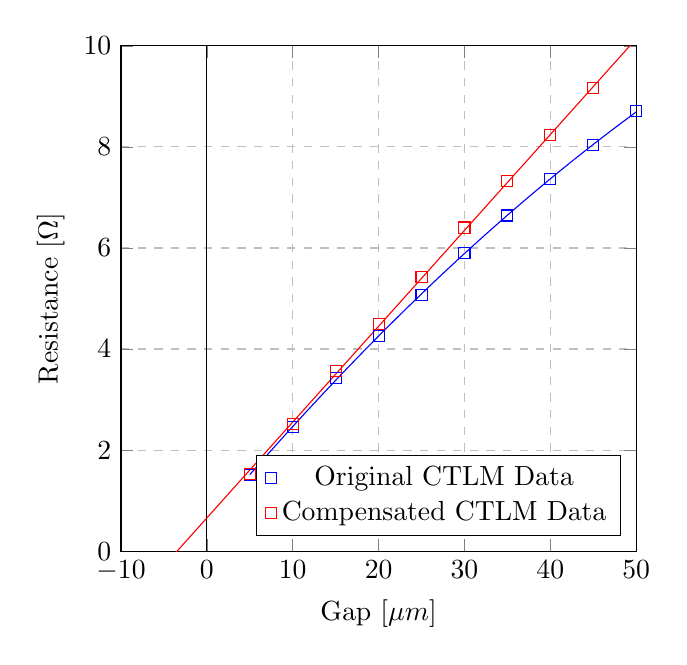
\begin{tikzpicture}

\begin{axis}[
    %title={Temperature dependence of CuSO$_4\cdot$5H$_2$O solubility},
    xlabel={Gap [$\mu m$]},
    ylabel={Resistance [$\Omega$]},
    height=8cm,
    width=0.67\textwidth,
    xmin=-10, xmax=50,
    ymin=0, ymax=10,
    xtick={-10, 0, 10, 20, 30, 40, 50},
    ytick={0, 2, 4, 6, 8, 10},
    % extra y ticks       = 0,
    % extra y tick labels = ,
    % extra y tick style  = { grid = major },
    legend pos=south east,
    ymajorgrids=true,
    xmajorgrids=true,
    grid style=dashed,
]

\addplot[color=blue, mark=square, only marks]
  coordinates {
  (5,1.505363832096823)
  (10,2.449740000726955)
  (15,3.421831099752043)
  (20,4.26394152103118)
  (25,5.070137988413258)
  (30,5.897088680026425)
  (35,6.64208850217324)
  (40,7.356653937259235)
  (45,8.039941315513527)
  (50,8.704528583743103)
};
  \addlegendentry{Original CTLM Data}

\addplot[color=red, mark=square, only marks]
    coordinates {
      (5,1.5245819322833463)
      (10,2.5136557475645573)
      (15,3.5587516564503536)
      (20,4.4966681982956205)
      (25,5.424233303346553)
      (30,6.403332285388977)
      (35,7.323979842935674)
      (40,8.242064238392762)
      (45,9.157502883492521)
      (50,10.085819749510799)
  };
    \addlegendentry{Compensated CTLM Data}

\addplot[color=black]
  coordinates{
    (0,0)
    (0,10)};


\addplot[color=blue,samples=100][domain=5:50]{-0.00077678*x^2 + 0.20218898*x + 0.5225879};

\addplot[color=red,samples=100][domain=-10:50]{0.18961899*x + 0.65853675};

\addplot[color=black] coordinates{(0,0) (10,0)};


\end{axis}
\end{tikzpicture}

\caption{Plot of resistance against CTLM gap size with the as measured data in blue and the data with the correction factor shown in \ref{eq:correction} applied shown in red. From the graph $2L_T = 3.473\mu m$, $2R_c = 0.659\Omega$, and $\rho_0 = $\hl{.......}}
\label{fig:ctlm_res}
\end{center}
\end{figure}


% \hl{6.25\%
%
% Plot CTLM results for one device from your group. Why do we use CTLMs over TLMs? Describe the salient features of the graph, and comment on any relationship to previous plots. Comment on why only the p-contact is analysed. [150 words max + Figures]}

Figures \ref{fig:ctlms_iv} shows the I-V plot for all gap size measurements from the circular transfer length method (CTLM). The CTLMs had a radius of $200\mu m$ and gap sizes from 5 to $50\mu m$ in steps of $5\mu m$. The plots for all gap sizes are close to linear implying that the contacts have an ohmic response.

The average resistance for each gap was found and plotted against the gap sizes, see figure \ref{fig:ctlm_res}. The true gap sizes were not measured and are assumed to be exactly as designed. Due to the nature of CTLMs, the radii of the two contacts cannot be equal. It is therefore necessary to include a correction factor which is found using equation \ref{eq:correction}

\begin{equation}
  C = \frac{1}{R_1}ln(\frac{R_1 + S}{R_1})
  \label{eq:correction}
\end{equation}

When the line of best fit for the corrected resistance values, shown in red, on figure \ref{fig:ctlm_res} are extrapolated it is found that the resistance values when the gap size is $0\mu m$ the resistance is $0.659\Omega$. This is equivalent to $2R_c$.
